\bartchapterimage{heic1107a.jpg}
\chapter{Special functions}
\bartthumb{heic1107a.png}
\label{cha:gamma}
%
\section{Legendre elliptic integral function}
%
\subsection{Introduction}
%
The Legendre elliptic integral function appears naturally when evaluationg
distances like the luminosity distance in a flat Universe. But the most of the
time, this function isn't used directly because of the difficulty of
implementation, and when it's already adapted, this is not for all kinds of
value. In following sections, we described how to use the NSWC implementation
of elliptic integrals.
%
\subsection{Luminosity distance}
%
Our goal is to easily and precisely compute the luminosity distance given a
cosmology according to the formula:
%
\begin{equation}
    d_L(z)=\cfrac{c(1+z)}{H_0}\int_0^z\cfrac{\dd{t}}{\sqrt{\Omega_m{(1+t)}^3+\Omega_\Lambda}}
\end{equation}
%
Making the change of variable $u=1/t$ and defining
$s=\sqrt{3}{(1-\Omega_m)/\Omega_m}$ gives us:
%
\begin{equation}
    d_L(z)=\cfrac{c(1+z)}{H_0\sqrt{s\Omega_m}}\left[T(s)-T\left(\cfrac{s}{1+z}\right)\right]
\end{equation}
%
with
%
\begin{equation}
    T(x)=\int_0^x\cfrac{\dd{u}}{\sqrt{u^4+u}}
\end{equation}

As described in \citet{Liu+11}, this integral is an elliptic integral, and such
integrals can be expressed in terms of Carlson symmetric forms
$R_F(x_1,x_2,x_3)$:
%
\begin{equation}
    R_F(x_1,x_2,x_3)=\cfrac{1}{2}\int_0^\infty\cfrac{\dd{t}}{\sqrt{(t+x_1)(t+x_2)(t+x_3)}}
\end{equation}
%
With help of the reduction theorem, we can write: \comments{I can't remember
how to do the computation. Some boring day, do it again for fun!}
%
\begin{equation}
    T(x)=4R_F(m,m+3+2\sqrt{3},m+3-2\sqrt{3})
\end{equation}
%
where
%
\begin{equation}
    m(x)=\cfrac{2\sqrt{x^2-x+1}}{x}+\cfrac{2}{x}-1
\end{equation}
%
\subsection{Algorithm}
%
\section{Incomplete gamma function}
\label{sec:gamma}
%
\subsection{Introduction}
%
By default, many algorithm used to compute incomplete gamma function doesn't
allowed to have negative parameters. By definition, the incomplete gamma
function $\Gamma\left({a,x}\right)$ is:
%
\begin{equation}
    \Gamma\left({a,x}\right)=\int_x^\infty{e^{-t}{t^{a-1}}\dd{t}}
\end{equation}
%
when $a\leq0$, we can't compute this function with usual algorithms. Moreover,
we need to used an algorithm which doesn't use the ``simple'' gamma function
$\Gamma\left({a}\right)$:
%
\begin{equation}
    \Gamma\left({a}\right)=\int_0^\infty{e^{-t}{t^{a-1}}\dd{t}}
\end{equation}
%
Indeed this function have singularities for negative values of $a$ where $a$ is
an integer, as we can see in figure (\ref{fig:gamma}).
%
\begin{figure}[hbtp]
    \centering
    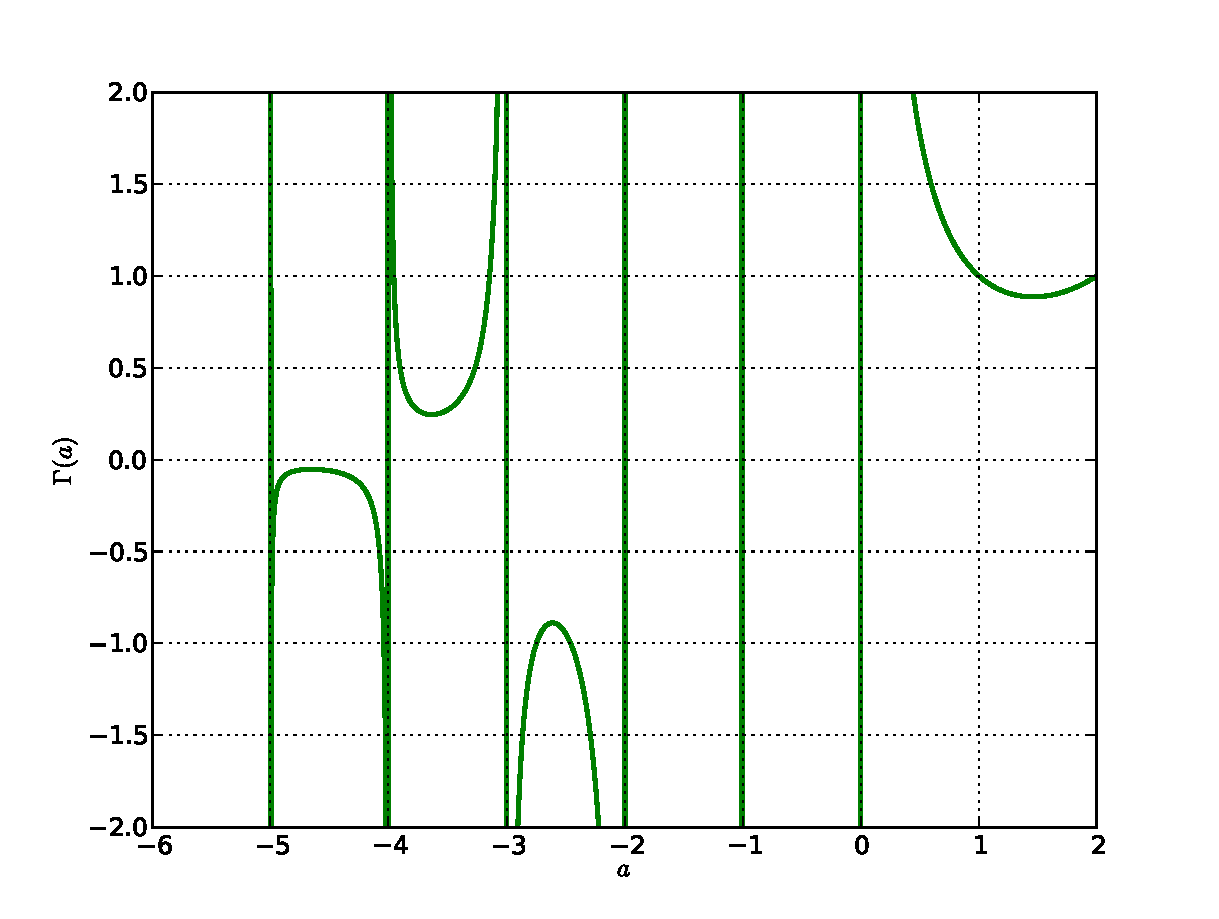
\includegraphics[width=0.5\linewidth]{figures/gamma/gamma}
    \caption{The gamma function.\label{fig:gamma}}
\end{figure}
%
So we need an algorithm which not involves to use the gamma function for
negative values. Here is described such algorithm.
%
\subsection{Algorithm}
%
\subsubsection{Theory}
%
The best way to compute the incomplete gamma function for $a$ negative values
is to use recurrence relations. Let us define:
%
\begin{equation}
    \Gamma\left({a+1,x}\right)=\int_x^\infty{e^{-t}{t^{a}}\dd{t}}
\end{equation}
%
Defining $u'=e^{-t}$ and $v=t^a$, we can use integration by parts:
%
\begin{equation}
    \Gamma\left({a+1,x}\right)={\left[-e^{-t}{t^a}\right]}_x^\infty + a \int_x^\infty{e^{-t}{t^{a-1}}\dd{t}}
\end{equation}
%
The all integrated part is always zero for all values of $a$ at infinity, and
the second member of the right hand side of the previous equation lets appear
the definition of the incomplete gamma function. So the recurrence relation for
the incomplete gamma function is:
%
\begin{equation}
    \Gamma\left({a+1,x}\right)=e^{-x}{x^a} + a \Gamma\left({a,x}\right)
\end{equation}
%
We can see that computing the incomplete gamma function for $a<=0$ can be done
with a recursive function using the function at higher values of $a$.
%
\begin{equation}
    \Gamma\left({a,x}\right)= \cfrac{\Gamma\left({a+1,x}\right) - e^{-x}{x^a}}{a}
\end{equation}
%
The previous equation shows that there is still a problem for integer values of
$a$ because if $a=-2$ for example, at a moment in the recursion, we have a
value of 0 for $a$ which create problems. If we refer to
\citet{abramowitz+stegun}, the definition of the elliptical integral is:
%
\begin{equation}
    E_n\left({z}\right)=\int_1^\infty{e^{-zt}}{t^{-n}}\dd{t}
\end{equation}
%
for integer values of $n$. If we change the variable in the integral to
$t'=zt$, we can rewrite the equation to have:
%
\begin{equation}
    E_n\left({z}\right)={z^{n-1}}\Gamma\left({1-n,z}\right)
\end{equation}
%
so:
%
\begin{equation}
    \Gamma\left({a,x}\right)={x^a}E_{1-a}\left({x}\right)
\end{equation}
%
for $a\leq0$ and $a$ integer. Now we have a good computation for the incomplete
gamma function. But numerically, there is still a problem near integer negative
values of $a$. If $a$ is very close to an integer value, at a moment in the
recursion, $a$ is very small. So $1/a$ can be bigger than the overflow value
for the machine. To avoid this, we add a condition for $a$ when it is near
zero.

An other definition of the incomplete gamma function is:
%
\begin{equation}
    \Gamma\left({a,x}\right)=\Gamma\left({a}\right)-\gamma\left({a,x}\right)=\Gamma\left({a}\right)\left({1-P\left({a,x}\right)}\right)
\end{equation}
%
with:
%
\begin{equation}
    \gamma\left({a,x}\right)=\int_0^x{e^{-t}{t^{a}}\dd{t}}
\end{equation}
%
In \citet{NumericalRecipes} exists a precise computation of the function
$P\left({a,x}\right)$. We can remark that this function isn't needed in the recursion
if we have already access to a function which compute the incomplete gamma
function for positive values of $a$.

Following is described the algorithm for computing incomplete gamma function
without loss of precision and without numericals problems for negative values
of $a$.
%
\subsubsection{Numerical}
%
\begin{minted}[bgcolor=griscode, linenos]{python}
def gammainc(a, x):

    """
    To compute the incomplete gamma function
    without loss of precision or without numerical
    problems. OF is the value of the overflow for
    the machine and expint( n, x ) the function
    which computes the integral function for n and x.
    """

    import numpy as np

    if x >= 0.:
        if a <= 1.:
            if a == int(a) or OF * abs(a) < 1 :
                return x ** int(a) * expint(1 - int(a), x)
            else :
                return (gammainc(a + 1, x) -
                    np.exp(-x) * (x ** a)) / a

        else :
            return gamma(a) (1 - P(a, x))
            # or call the function which computes
            # the incomplete gamma function for
            # positive values of a
\end{minted}
